\documentclass{uni_tue_template}

\usepackage{color}
\usepackage[colorlinks]{hyperref}
\definecolor{darkred}{rgb}{0.5,0,0}
\definecolor{darkgreen}{rgb}{0,0.5,0}
\definecolor{darkblue}{rgb}{0,0,0.7}
\hypersetup{
			linkcolor={darkblue},
			filecolor={darkgreen},
			urlcolor={darkred},
			citecolor={darkblue},
}

\usepackage[export]{adjustbox}
\usepackage{tikz}
\usetikzlibrary{shapes}
\usepackage{rotating}
\usepackage{sistyle}

\lstdefinestyle{sql}{%
	language=SQL,%
	commentstyle=\color{comment},%
	stringstyle=\color{string},%
	keywordstyle=\color{keyword}\bfseries,%
	morekeywords={text, real, begin},%
	basicstyle=\ttfamily\footnotesize,%
	numbers=left,
	numberstyle=\tiny\color{black},
	stepnumber=1,
	showstringspaces=true,%
	columns=fixed,%
	moredelim=[is][\itshape]{@@}{@@},%
	tabsize=2
}
\lstset{aboveskip=-.6cm,style=sql, firstline=4}

\newcommand{\otext}[1]{\overset{\mathclap{\rule[-.3\baselineskip]{0pt}{0cm}\textmd{#1}}}}
\newcommand{\set}[1]{\mathbb{#1}}
\newcommand{\code}[1]{\texttt{{\footnotesize #1}}}
\newcommand{\md}[1]{\textmd{#1}}

% content of left head area e.g. subject like ETI
\def \headLeft{Andreas Schmied (3087156),\newline Tobias Stumpp (3798377)}

% content of center head area, used for names
\def \names{\"Ubungsblatt 7,\\ Datenbanksysteme II}

% content of right head area e.g. semester like WiSe 2012/13
\def \headRight{\today}

% set name for exercises
\def \exerciseName{Aufgabe}

\begin{document}
\exercise{}\\
\emph{Gegeben sei der \emph{Extendible Hashing Index} in Abbildung \ref{fig:1}. Auf dieser Grundlage beantworten Sie bitte folgende Fragen:}
\subExBegin{1{.}}
  \item \emph{Was können Sie über den Eintrag, der als Letzter in diesen Index eingetragen wurde sagen, wenn Sie wissen, dass bis dato kein Eintrag gelöscht wurde? Könnte dieser Eintrag einen Split ausgelöst haben?}\\
  Nein, da bisher nur $A$ gesplittet wurde und hier aber mehr als $d+1=5$ Elemente vorhanden sind, weswegen der Split mehrere Eintragungen zurück liegt.  
  \item \emph{Zeichnen Sie den Index aus Abbildung $1$, nachdem Sie einen Eintrag $v$ mit dem Hash-Wert $68$ eingetragen haben.}
  \begin{figure}[h!]
    \centering
    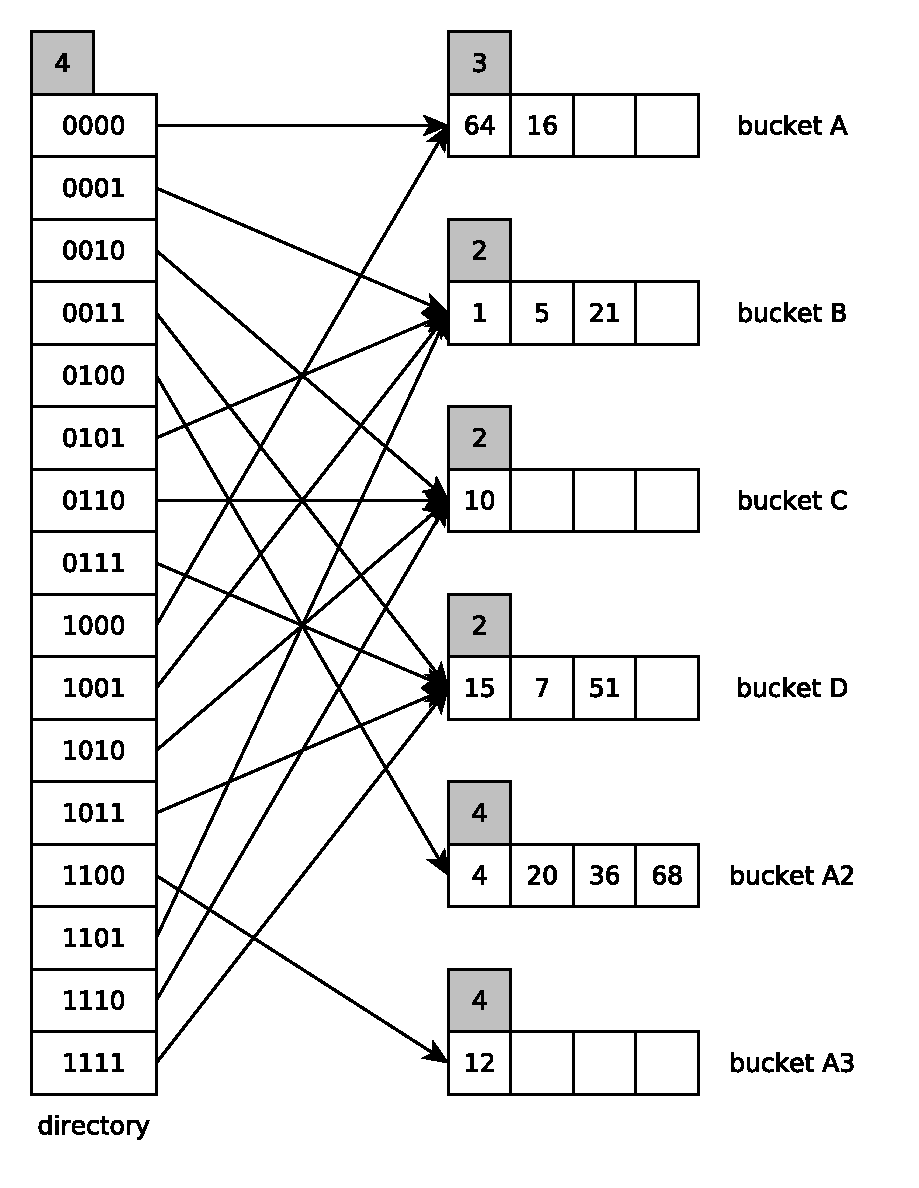
\includegraphics[scale=0.7]{graphml/01_2.pdf}
  \end{figure}
  \newpage
  \item \emph{Fügen Sie im originalen Index von Abbildung $1$ die Werte $v_1$ und $v_2$ mit den Hash-Werten $17$ und $69$ ein und zeichnen Sie den Index auf.}
  \begin{figure}[h!]
    \centering
    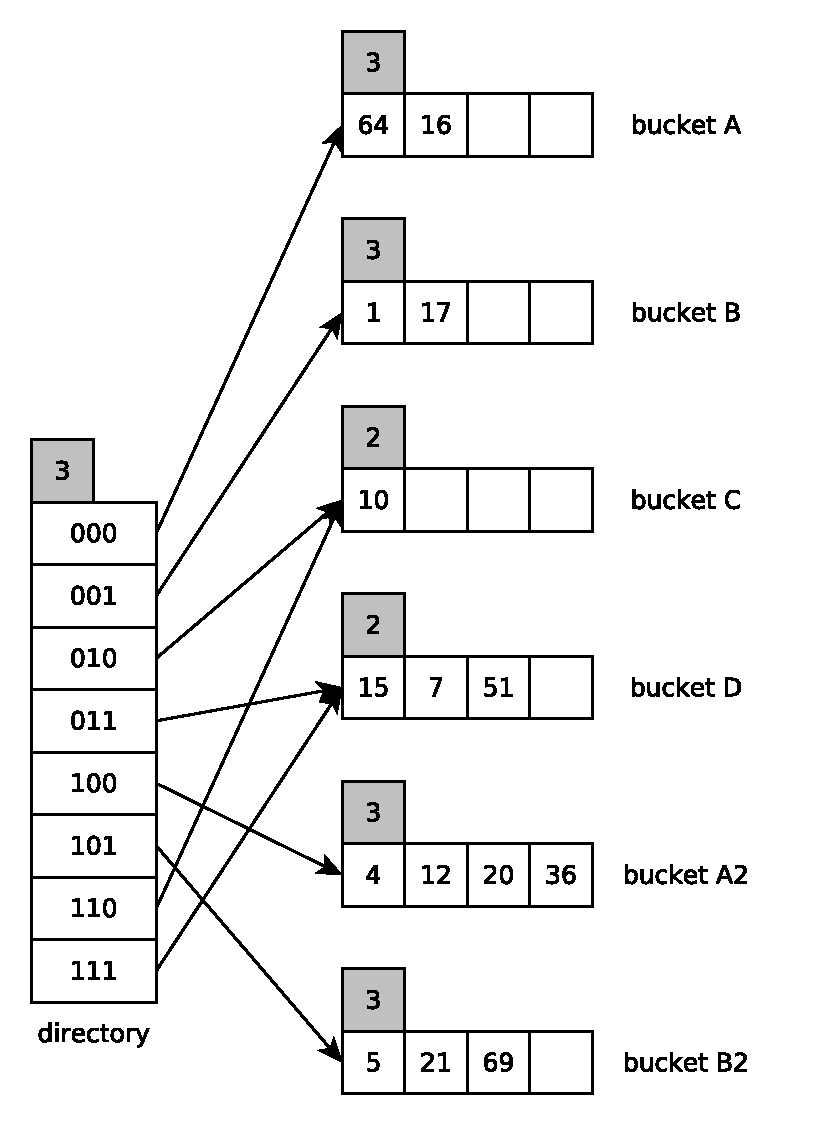
\includegraphics[scale=0.7]{graphml/01_3.pdf}
  \end{figure}
  \newpage
  \item \emph{Löschen Sie im Index von Abbildung $1$ den Eintrag mit dem Hash-Wert $21$.}
  \begin{figure}[h!]
    \centering
    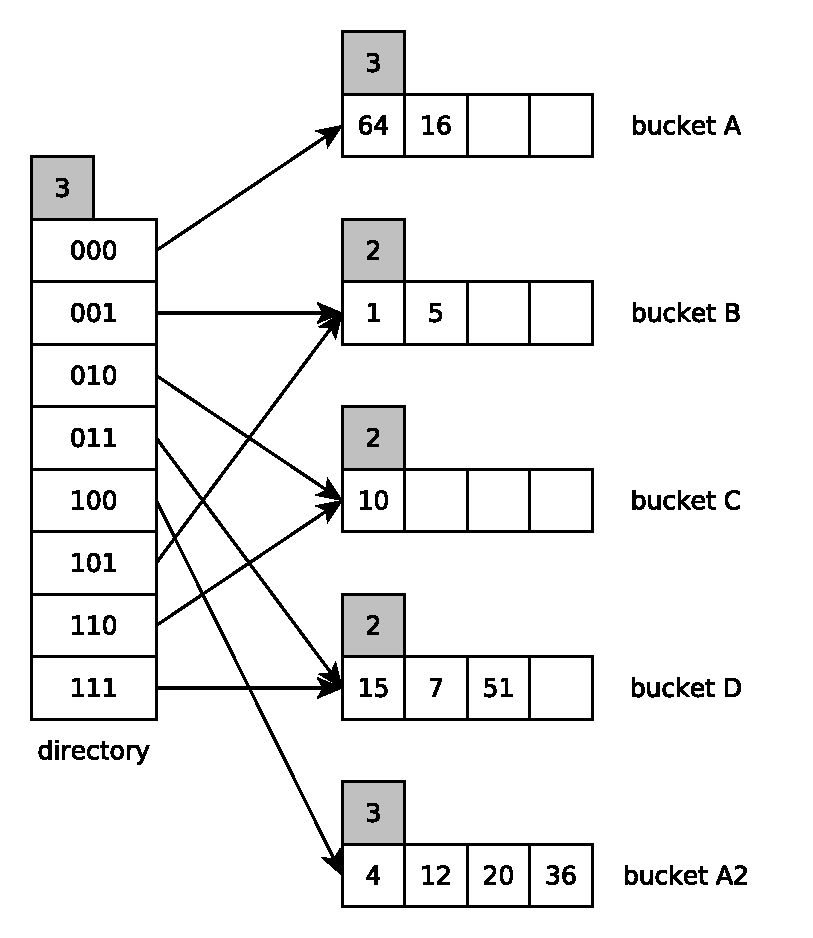
\includegraphics[scale=0.7]{graphml/01_4.pdf}
  \end{figure}
  \newpage
  \item \emph{Zeichnen Sie den Index aus Abbildung $1$, nachdem Sie den Eintrag mit dem Hash-Wert 10 gelöscht haben. Wird dadurch eine Verschmelzung ausgelöst? Wenn nicht, nennen Sie die Gründe dafür. (Beachten Sie, dass hier wieder der vollständige Löschalgorithmus zum Einsatz kommt.)}\\
  \begin{figure}[h!]
    \centering
    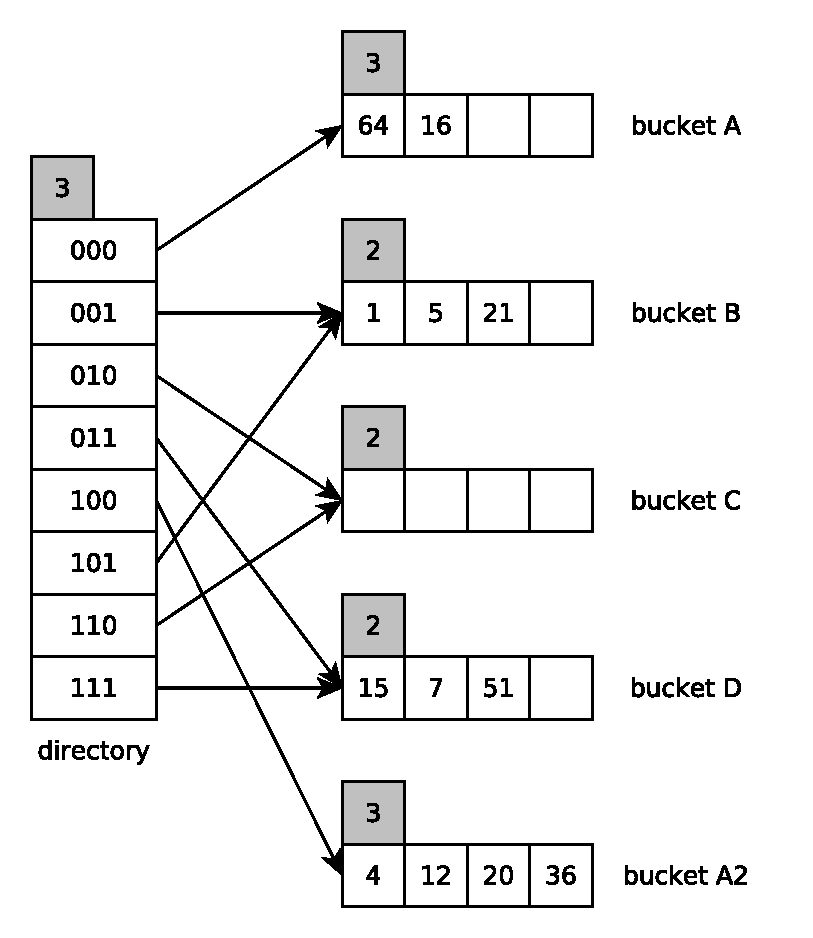
\includegraphics[scale=0.7]{graphml/01_5.pdf}
  \end{figure}\\
  Es wird keine Verschmelzung ausgelöst, da eine Verschmelzung Konflikte für Bucket $A$ und $A2$ auslösen. Anders ausgedrückt, die \emph{mininal verlangte} globale Größe $3$ ist größer, als die lokale Größe $2$.
  \newpage
\subExEnd{}
%
\newpage 
%
\exercise{}\\
\emph{Gegeben Sei der \emph{Linear Hashing Index} in Abbildung 2. Das Kriterium für einen Split ist das Anlegen einer neuen \emph{overflow page}.\\
Auf dieser Grundlage beantworten Sie bitte folgende Fragen:}
\subExBegin{1{.}}
  \item \emph{Was können Sie über den Eintrag, der als Letzter in diesen Index eingetragen wurde sagen, wenn Sie wissen, dass bis dato kein Eintrag gelöscht wurde? Könnte dieser Eintrag einen Split ausgelöst haben?}\\
  Ein durch den letzten Eintrag ausgelöster Split ist möglich, da die Page $0$ und $4$ zusammen $n+1=5$ Elemente ergeben, auch da der \code{next}$=1$ ist. 
  \item \emph{Zeichnen Sie den Index aus Abbildung $2$, nachdem Sie einen Eintrag $v$ mit dem Hash-Wert $4$ eingetragen haben.}
  \begin{figure}[h!]
    \centering
    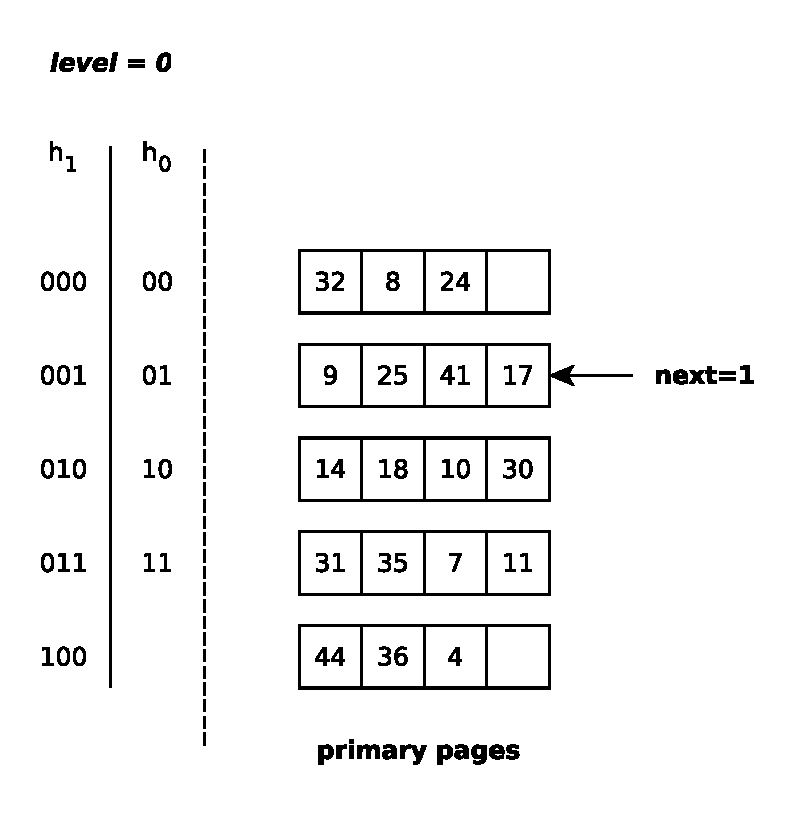
\includegraphics[scale=0.7]{graphml/02_2.pdf}
  \end{figure}
  \newpage
  \item \emph{Fügen Sie im originalen Index von Abbildung $2$ den Wert $v$ mit den Hash-Wert $15$ ein und zeichnen Sie den Index auf.}
  \begin{figure}[h!]
    \centering
    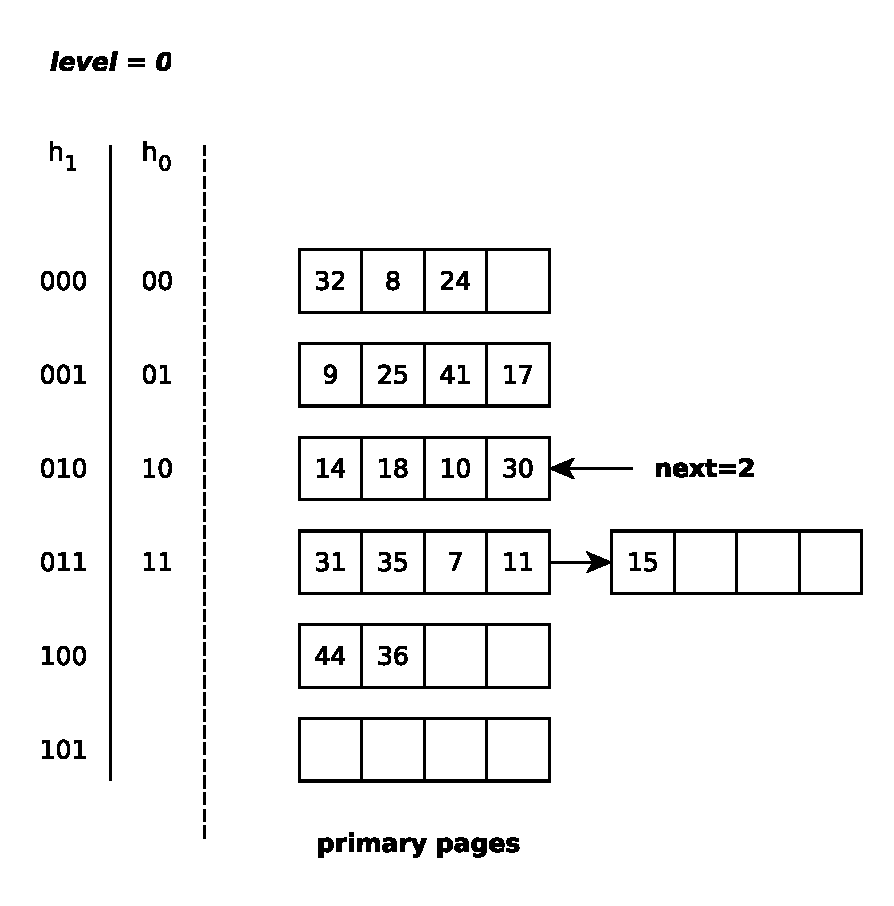
\includegraphics[scale=0.7]{graphml/02_3.pdf}
  \end{figure}
  \newpage
  \item \emph{Löschen Sie im Index von Abbildung $2$ die Einträge mit den Hash-Werten $36$ und $44$. Legen Sie dabei "empty primary bucket" als \emph{underflow} Kriterium zu Grunde.}
  \begin{figure}[h!]
    \centering
    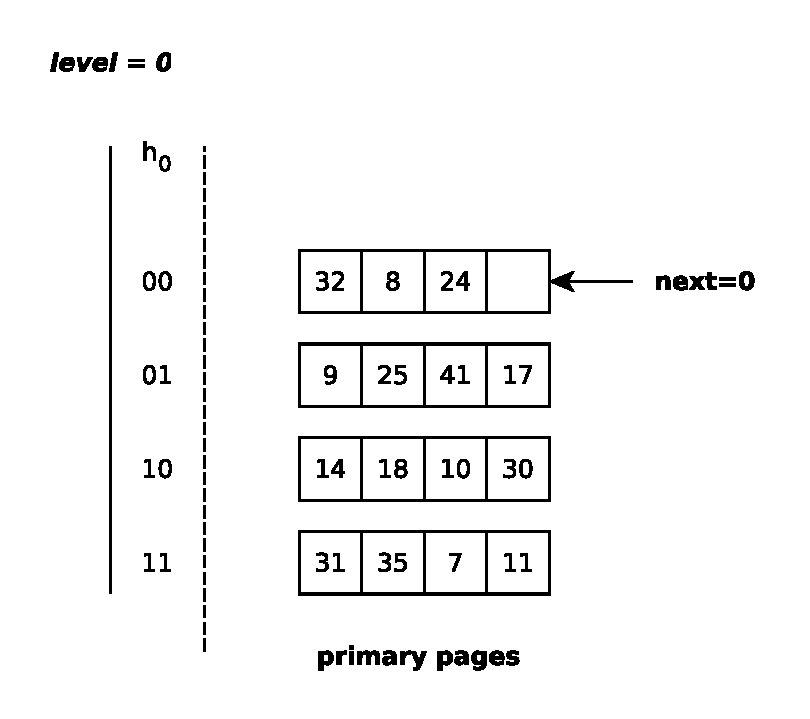
\includegraphics[scale=0.7]{graphml/02_4.pdf}
  \end{figure}
  \newpage
\subExEnd{}
%
\newpage 
%
\exercise{}\\
\emph{Gegeben sei eine Relation $R(a, b, c, d)$, die mit einer Million Tupeln gefüllt ist. $R$ ist als Heap-Datei mit unclustered Indizes organisiert. Die Tupel in $R$ seien in beliebiger Reihenfolge angeordnet. $a$ sei ein Kandidatenschlüssel für $R$, mit Werten zwischen $0$ bis $999999$. Für jede der folgenden Anfragen, geben Sie den Ansatz an welcher, die wenigsten I/O Operationen benötigt. Begründen Sie \emph{kurz}.}
\begin{itemize}
  \item \emph{Scannen der gesamten Heap-Datei.}
  \item \emph{Benutzen eines B+ Baumes auf das Attribut $a$.}
  \item \emph{Benutzen eines Hash-Index auf das Attribut $a$.}
\end{itemize}
Die Anfragen lauten wie folgt:
\subExBegin{1{.}}
  \item \hfill\\
\begin{lstlisting}
SELECT *
FROM R
\end{lstlisting}
  \item \hfill\\
\begin{lstlisting}
SELECT *
FROM R
WHERE a < 50
\end{lstlisting}
  \item \hfill\\
\begin{lstlisting}
SELECT *
FROM R
WHERE a = 50
\end{lstlisting}
  \item \hfill\\
\begin{lstlisting}
SELECT *
FROM R
WHERE a > 50 AND a < 100
\end{lstlisting}
\subExEnd{}
\subExBegin{1{.}}
  \item Scannen der gesamten Heap-Datei.\\
  Da ohnehin alle Elemente von $R$ gelesen werden überwiegt der sequential Scan in der Performanz gegenüber einem zusätzlichen Mehraufwand beim Durchlaufen der anderen Strukturen.
  \item Benutzen eines B+ Baumes auf das Attribut $a$.\\
  Bei Range-Queries haben B+ Bäume den geringsten Aufwand, da über die Baumstruktur eine schnelle Suche möglich ist und Querverweise das sequentielle Lesen ermöglichen. Sie bilden damit einen Kompromiss zwischen Heap-Scan und Index-Zugriff.
  \item Benutzen eines Hash-Index auf das Attribut $a$.\\
  Es wird nur ein Element gelesen, womit sich der Aufwand auf den Index-Zugriff beschränkt, hierbei ist der Hash-Index mit den wenigsten I/O's berechnet.
  \item Benutzen eines B+ Baumes auf das Attribut $a$.\\
  Bei Range-Queries haben B+ Bäume den geringsten Aufwand, da über die Baumstruktur eine schnelle Suche möglich ist und Querverweise das sequentielle Lesen ermöglichen. Sie bilden damit einen Kompromiss zwischen Heap-Scan und Index-Zugriff.
\subExEnd{}

\end{document}